\section{Simulation Analysis}

\subsection{Nodal Analysis at t < 0}
For the first part, as mentioned in the theoretical analysis, because the system has stabilized, we expect that for a long period of time no current will pass through the capacitor. The values obtained for this are presented in Tab. \ref{tab:ngs_norm}.

    \begin{table}[H]
    \centering
    \small
    \begin{tabular}{|c|c|c|c|}
          \hline
          Node/Branch & $@(i) [A]/ v [V]$\\
          \hline
          @gb[i] & -2.82647e-04\\ \hline
@id[current] & 1.016742e-03\\ \hline
@r1[i] & -2.69487e-04\\ \hline
@r2[i] & -2.82647e-04\\ \hline
@r3[i] & -1.31599e-05\\ \hline
@r4[i] & -1.17175e-03\\ \hline
@r5[i] & -1.29939e-03\\ \hline
@r6[i] & 9.022631e-04\\ \hline
@r7[i] & 9.022631e-04\\ \hline
v(1) & 7.795262e+00\\ \hline
v(2) & 7.515011e+00\\ \hline
v(3) & 6.927322e+00\\ \hline
v(4) & 2.756787e+00\\ \hline
v(5) & 7.555303e+00\\ \hline
v(6) & 1.145524e+01\\ \hline
v(7) & 9.222643e-01\\ \hline
cfp1 & 9.222643e-01\\ \hline

          \hline
    \end{tabular}
    \caption{Tension and current for every branch and node of the circuit for the stable solution when $V_s$ is stable.}
    \label{tab:ngs_norm}
    \end{table}
    
As we can see, the current value in the conductor is 0, which goes according to the expectations, i.e, for a long period of time, the charge accumulates there and the potential difference in the capacitor is equal to the potential difference that is coming in from the circuit, which means no current is pulled to it. The rest of the values are equal to the ones obtained in the theoretical analysis.

\subsection{$R_{eq}$ and time constant $\tau$}

The only thing that needed change from the previous subsection was the value for $V_s$, that changes to 0, in order to determine the $R_{eq}$ and that way $\tau$.

    \begin{table}[H]
    \centering
    \small
    \begin{tabular}{|c|c|c|c|}
          \hline
          Node/Branch & $@(i) [A]/ v [V]$\\
          \hline
          @gb[i] & 8.369438e-18\\ \hline
@r1[i] & 7.979758e-18\\ \hline
@r2[i] & -8.36944e-18\\ \hline
@r3[i] & 3.896799e-19\\ \hline
@r4[i] & -1.73508e-18\\ \hline
@r5[i] & -2.79994e-03\\ \hline
@r6[i] & 1.301043e-18\\ \hline
@r7[i] & 8.876953e-19\\ \hline
v(1) & 0.000000e+00\\ \hline
v(2) & 8.298505e-15\\ \hline
v(3) & 2.570053e-14\\ \hline
v(5) & 7.105427e-15\\ \hline
v(6) & 8.403629e+00\\ \hline
v(7) & -2.64534e-15\\ \hline
v(8) & -3.55271e-15\\ \hline
cfp1 & -2.64534e-15\\ \hline

          \hline
    \end{tabular}
    \caption{Tension and current for every branch and node of the circuit for the stable solution when $V_s$ is null.}
    \label{tab:ngs_tau}
    \end{table}
As we can see in Tab. \ref{tab:ngs_tau}, the values for the currents are practically 0 for every branch, excepting the currents going through $R_5$, $C_1$ and $V_d$ which, although are not presented in the table, one can easily see from the nodes tensions, specially for the tension in node 6. The result for node 6 in the theoretical analysis was $V_6 = 8.40363V$ while here is $V_6 = 8.403629V$, which represents but an approximation in octave. $I_5 = -2.79994\times 10^{-3} A$, $I_b \approx 0 A$, which means that $I_x = 2.79994\times 10^{-3} A$ while in the theoretical analysis we got $I_x = 2.80mA$, thus once again is but an approximation from Octave. This means that $R_{eq} = 3.0014k\Omega$. This means that the value for $\tau$ is the same as in the theoretical analysis.

\subsection{Natural solution for $v_6(t)$}

To simulate that the circuit was active since infinite, we use initial conditions has suggested by the teacher, while zeroing the voltage source $v_s$, which results in what is shown in Fig. \ref{fig:ngspice_c}

\vspace{-13mm}
\begin{figure}[H]
    \centering
    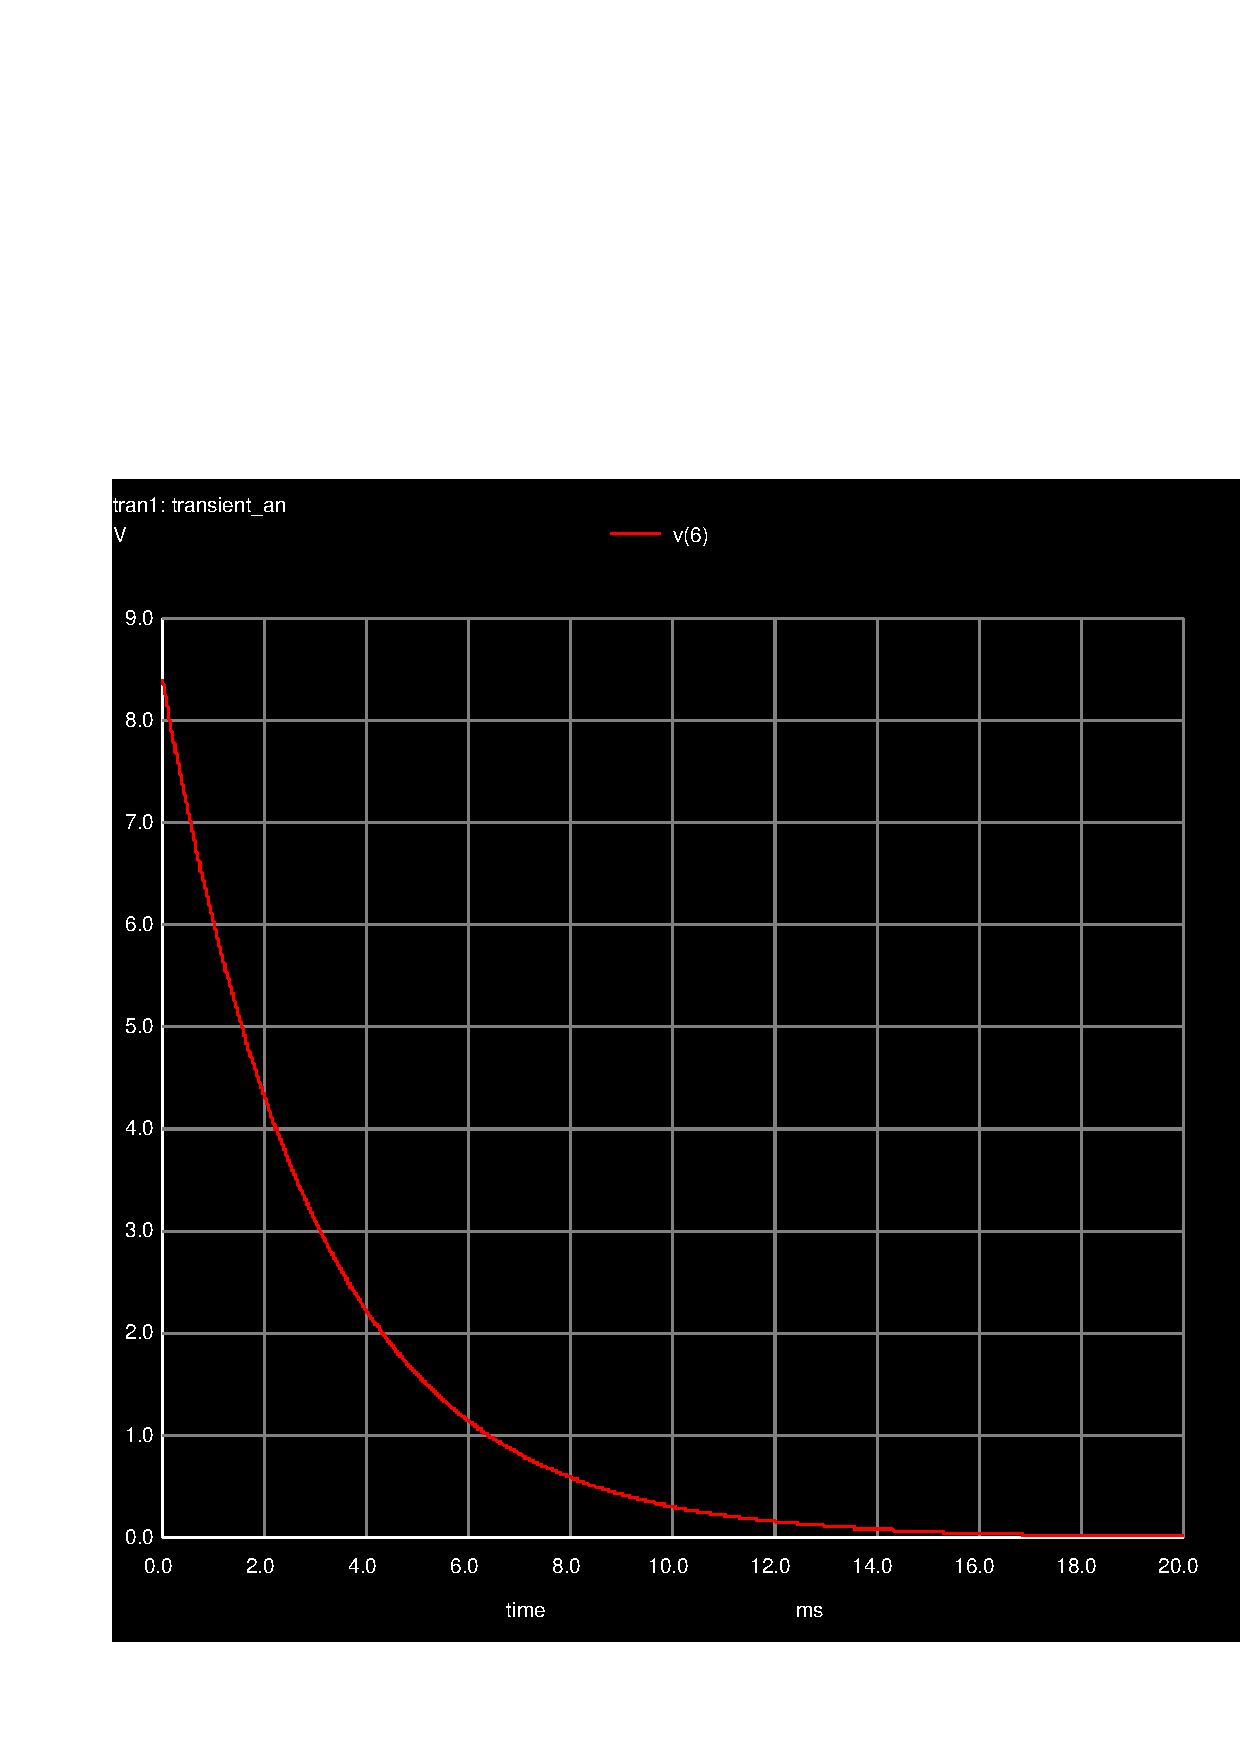
\includegraphics[width = 0.85\linewidth]{../sim/trans3.pdf}
        \caption{\textit{Natural solution for $v_s = 0$, having been charged, the capacitor, previously, since infinite (due to initial conditions).}}
    \label{fig:ngspice_c}
\end{figure}

This result is the same, as expected, as the one in Fig. \ref{fig:natural}.

\subsection{Forced solution for $v_6(t)$}

Having given no initial conditions and putting $v_s = sin(2\pi ft)$, we get the shown in Fig. \ref{fig:ngspice_d}. One should notice that this graph is not exactly the same as the one in Fig. \ref{fig:forced}, because here the system is behaving as if it were in the real world. What this means is that the voltage source starts by immediately having that sinusoidal behavior but it still is not in equilibrium with the rest of the circuit, which means that $v_6$ goes through a transient state first, before reaching the steady state form, in those initial milliseconds.

\vspace{-13mm}
\begin{figure}[H]
    \centering
    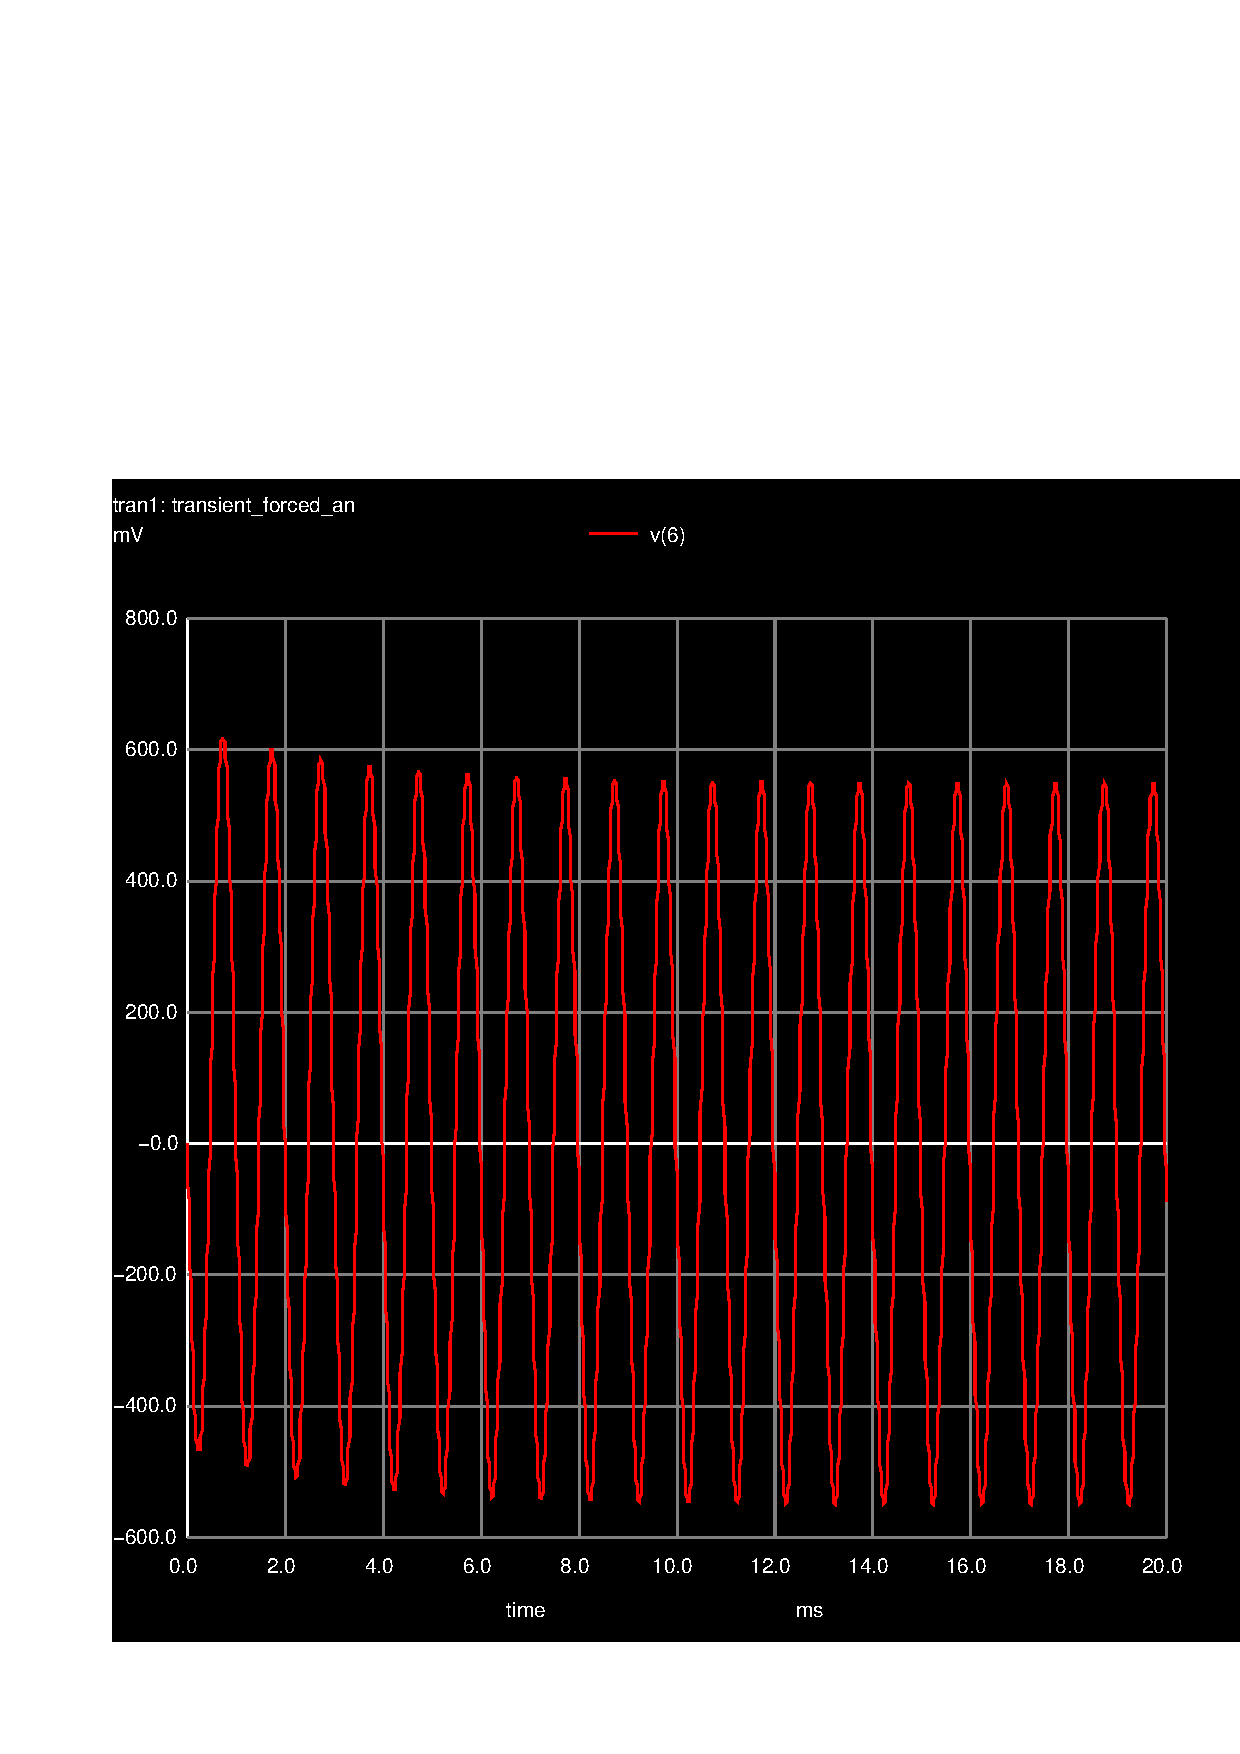
\includegraphics[width = 0.85\linewidth]{../sim/trans4.pdf}
        \caption{\textit{Forced solution for $v_s = sin(2\pi ft)$, having zero initial conditions, i.e., capacitor totally discharged.}}
    \label{fig:ngspice_d}
\end{figure}

If we want to add the forced and natural solution to get the real solution, we do the same for this part, but impose the initial conditions from the previous section. Thus, the result is what is shown in Fig. \ref{fig:ngspice_e}, in red. In the same figure, in blue, one can see the voltage source behavior as well. As discussed in the theoretical analysis, the voltage source and $v_6$ are totally out of phase, which only means that the current takes some time to be "felt" in node 6.

\vspace{-13mm}
\begin{figure}[H]
    \centering
    \includegraphics[width = 0.85\linewidth]{../sim/trans5.pdf}
        \caption{\textit{Sum of forced and natural solution in red and $v_s$ in red.}}
    \label{fig:ngspice_e}
\end{figure}

As asked in the powerpoint, it is also shown the behaviour of t$V_x$ in the sum of the two solutions, as shown in Fig. \ref{fig:ngspice_f}.

\vspace{-13mm}
\begin{figure}[H]
    \centering
    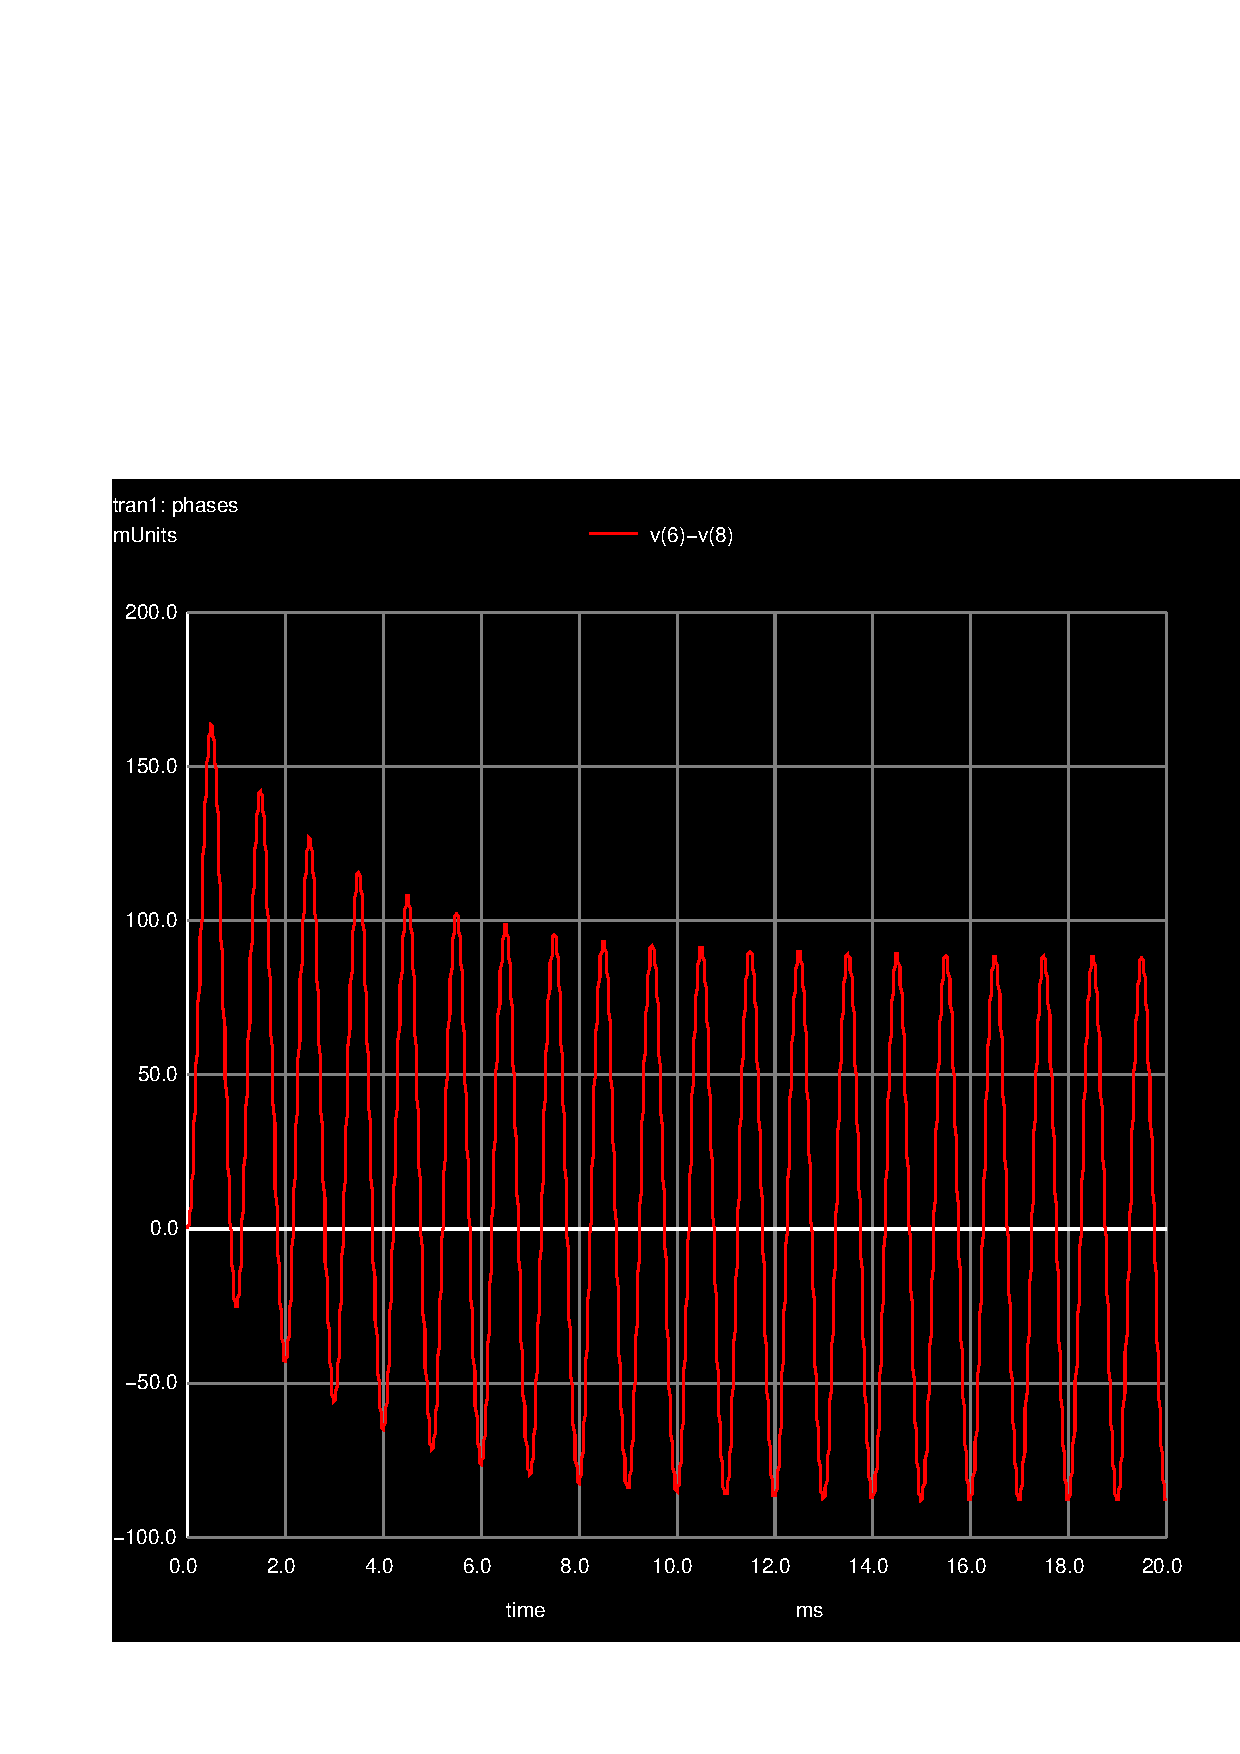
\includegraphics[width = 0.85\linewidth]{../sim/trans6.pdf}
        \caption{\textit{Sum of forced and natural solution for $v_x$.}}
    \label{fig:ngspice_f}
\end{figure}

All of the graphs are according to the theoretical analysis.

\subsection{Magnitude and Phase as Functions of Frequency}

The magnitude as a function of the frequency for several variables, in dB, is shown in Fig. \ref{fig:magnitude_spice}.

\vspace{-13mm}
\begin{figure}[H]
    \centering
    \includegraphics[width = 0.85\linewidth]{../sim/voltage_mag.pdf}
        \caption{\textit{Magnitudes of $v_6$ (orange), $v_6 - v_8$ (red) and $v_s$ (blue) as a function of frequency.}}
    \label{fig:magnitude_spice}
\end{figure}

As expected, the magnitudes for $v_6$ and $v_6 - v_8$ start by accompanying the behaviour of the circuit but, for frequencies that are greater than 1000Hz, the system saturates and it no longer has the ability to go accordingly to the voltage source. Thus, due to saturation, the potential difference goes to zero, and the singular voltage for node 6 stabilizes at a certain value of saturation. One expects always that the magnitude of the source with respect to itself to be the same, thus, because it is a logarithmic scale, it is 0, as seen. For the phases response, check Fig. \ref{fig:ngspice_phase}.

\vspace{-13mm}
\begin{figure}[H]
    \centering
    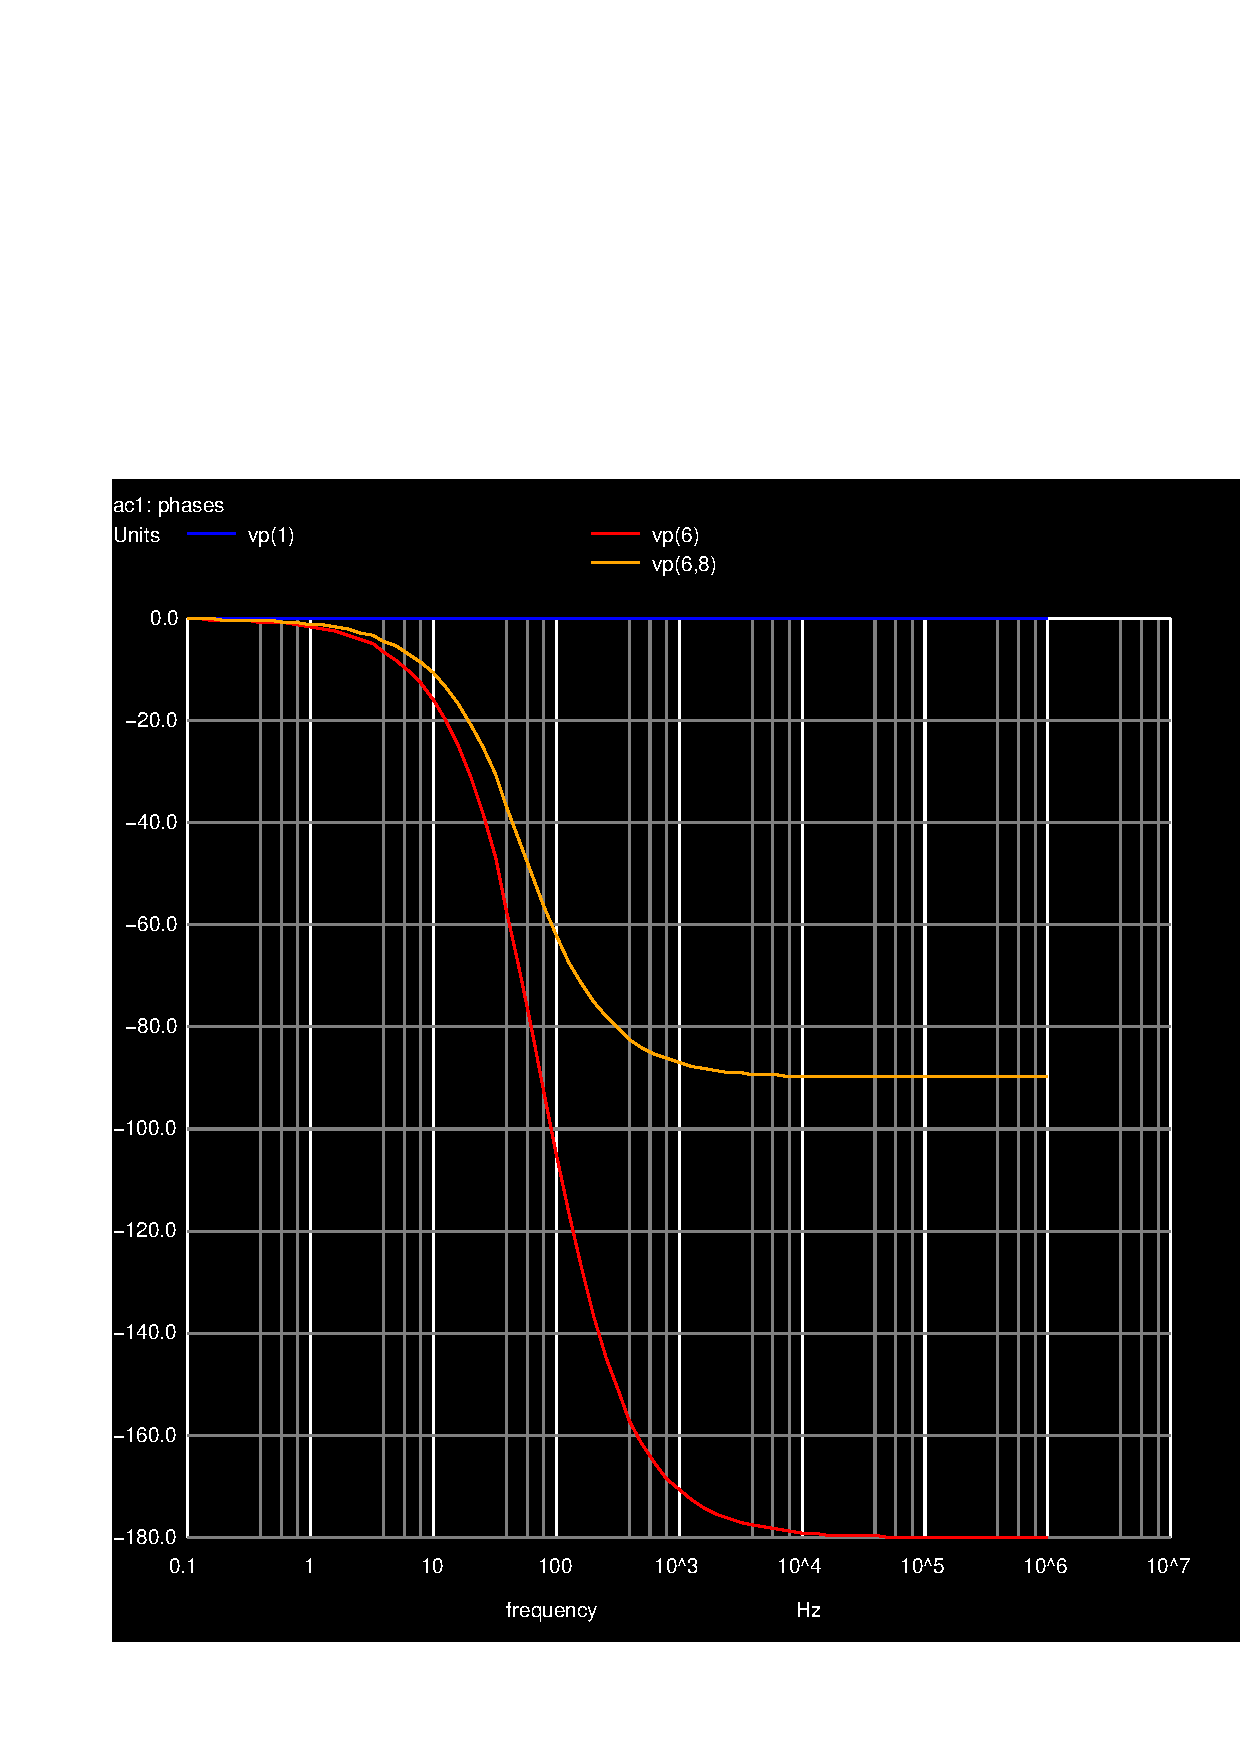
\includegraphics[width = 0.85\linewidth]{../sim/zezoca.pdf}
        \caption{\textit{Phases of $v_6$ (red), $v_6 - v_8$ (orange) and $v_s$ (blue) as a function of frequency.}}
    \label{fig:ngspice_phase}
\end{figure}

The main difference in Fig. \ref{fig:ngspice_phase} to Fig. \ref{fig:phase} is the base level, i.e., the voltage level. Octave assumes it to be $-\pi/2$, while ngspice rightly sets it to 0. However, the evolution of the phases throughout time is equivalent. This concludes our simulation analysis.